\chapter{Demo}
\label{sec:demo}       % labels can be put almost anywhere and can be referencef from anywhere.
Write some useful intro. Here are tips along the way:

\section{Tips}
\subsection{How to Describe}
% optional: set the spacing between columns
\setlength{\columnsep}{30 pt}
When listing several points you have three basic options:
\begin{multicols}{3}
    \begin{itemize}
        \item itemize
        \item enumerate
        \item description
    \end{itemize}

    \vfill\null
    \columnbreak

    \begin{enumerate}
        \item itemize
        \item enumerate
        \item description
    \end{enumerate}

    \vfill\null
    \columnbreak

    \begin{description}
        \item[itemize] short, unordered
        \item[enumerate] short ordered
        \item[description] listing of descriptions. Also nice for longer ones.
    \end{description}

\end{multicols}


\subsection{How to Quote}

\begin{quote}
    "This is a quote!"
\end{quote}

\begin{itemize}
    \item Citations to a source can be made like this \verb|\cite{gratl17task}| =~\cite{gratl17task}
          \subitem Always join text and the citation with a non-breaking space: \verb|text~\cite{foo}|.
    \item Referencing Sections, Figures, Tables, Formulas: \verb|\autoref{sec:demo}| = \autoref{sec:demo}.
    \item Footnotes for url or further notes: \verb|\footnote{\url{https://www.top500.org}}| = \footnote{\url{https://www.top500.org}}
\end{itemize}

\subsection{How to Math}

Use the align environment for equations especially if you want to align them somehow.

\begin{align}
    1 + 1                          & \ne 3 \\
    \left(\dfrac{10}{1}\right) - 9 & = 1
\end{align}

% if you need a pagebreak because figure placement is broken:
\clearpage

\section{Environments}

\subsection{How to Figure}

Anything can also be put in multiple columns.

\begin{multicols}{2} % defines an environment with two columns
    \begin{figure}[H] % [H] for HERE
        \centering
        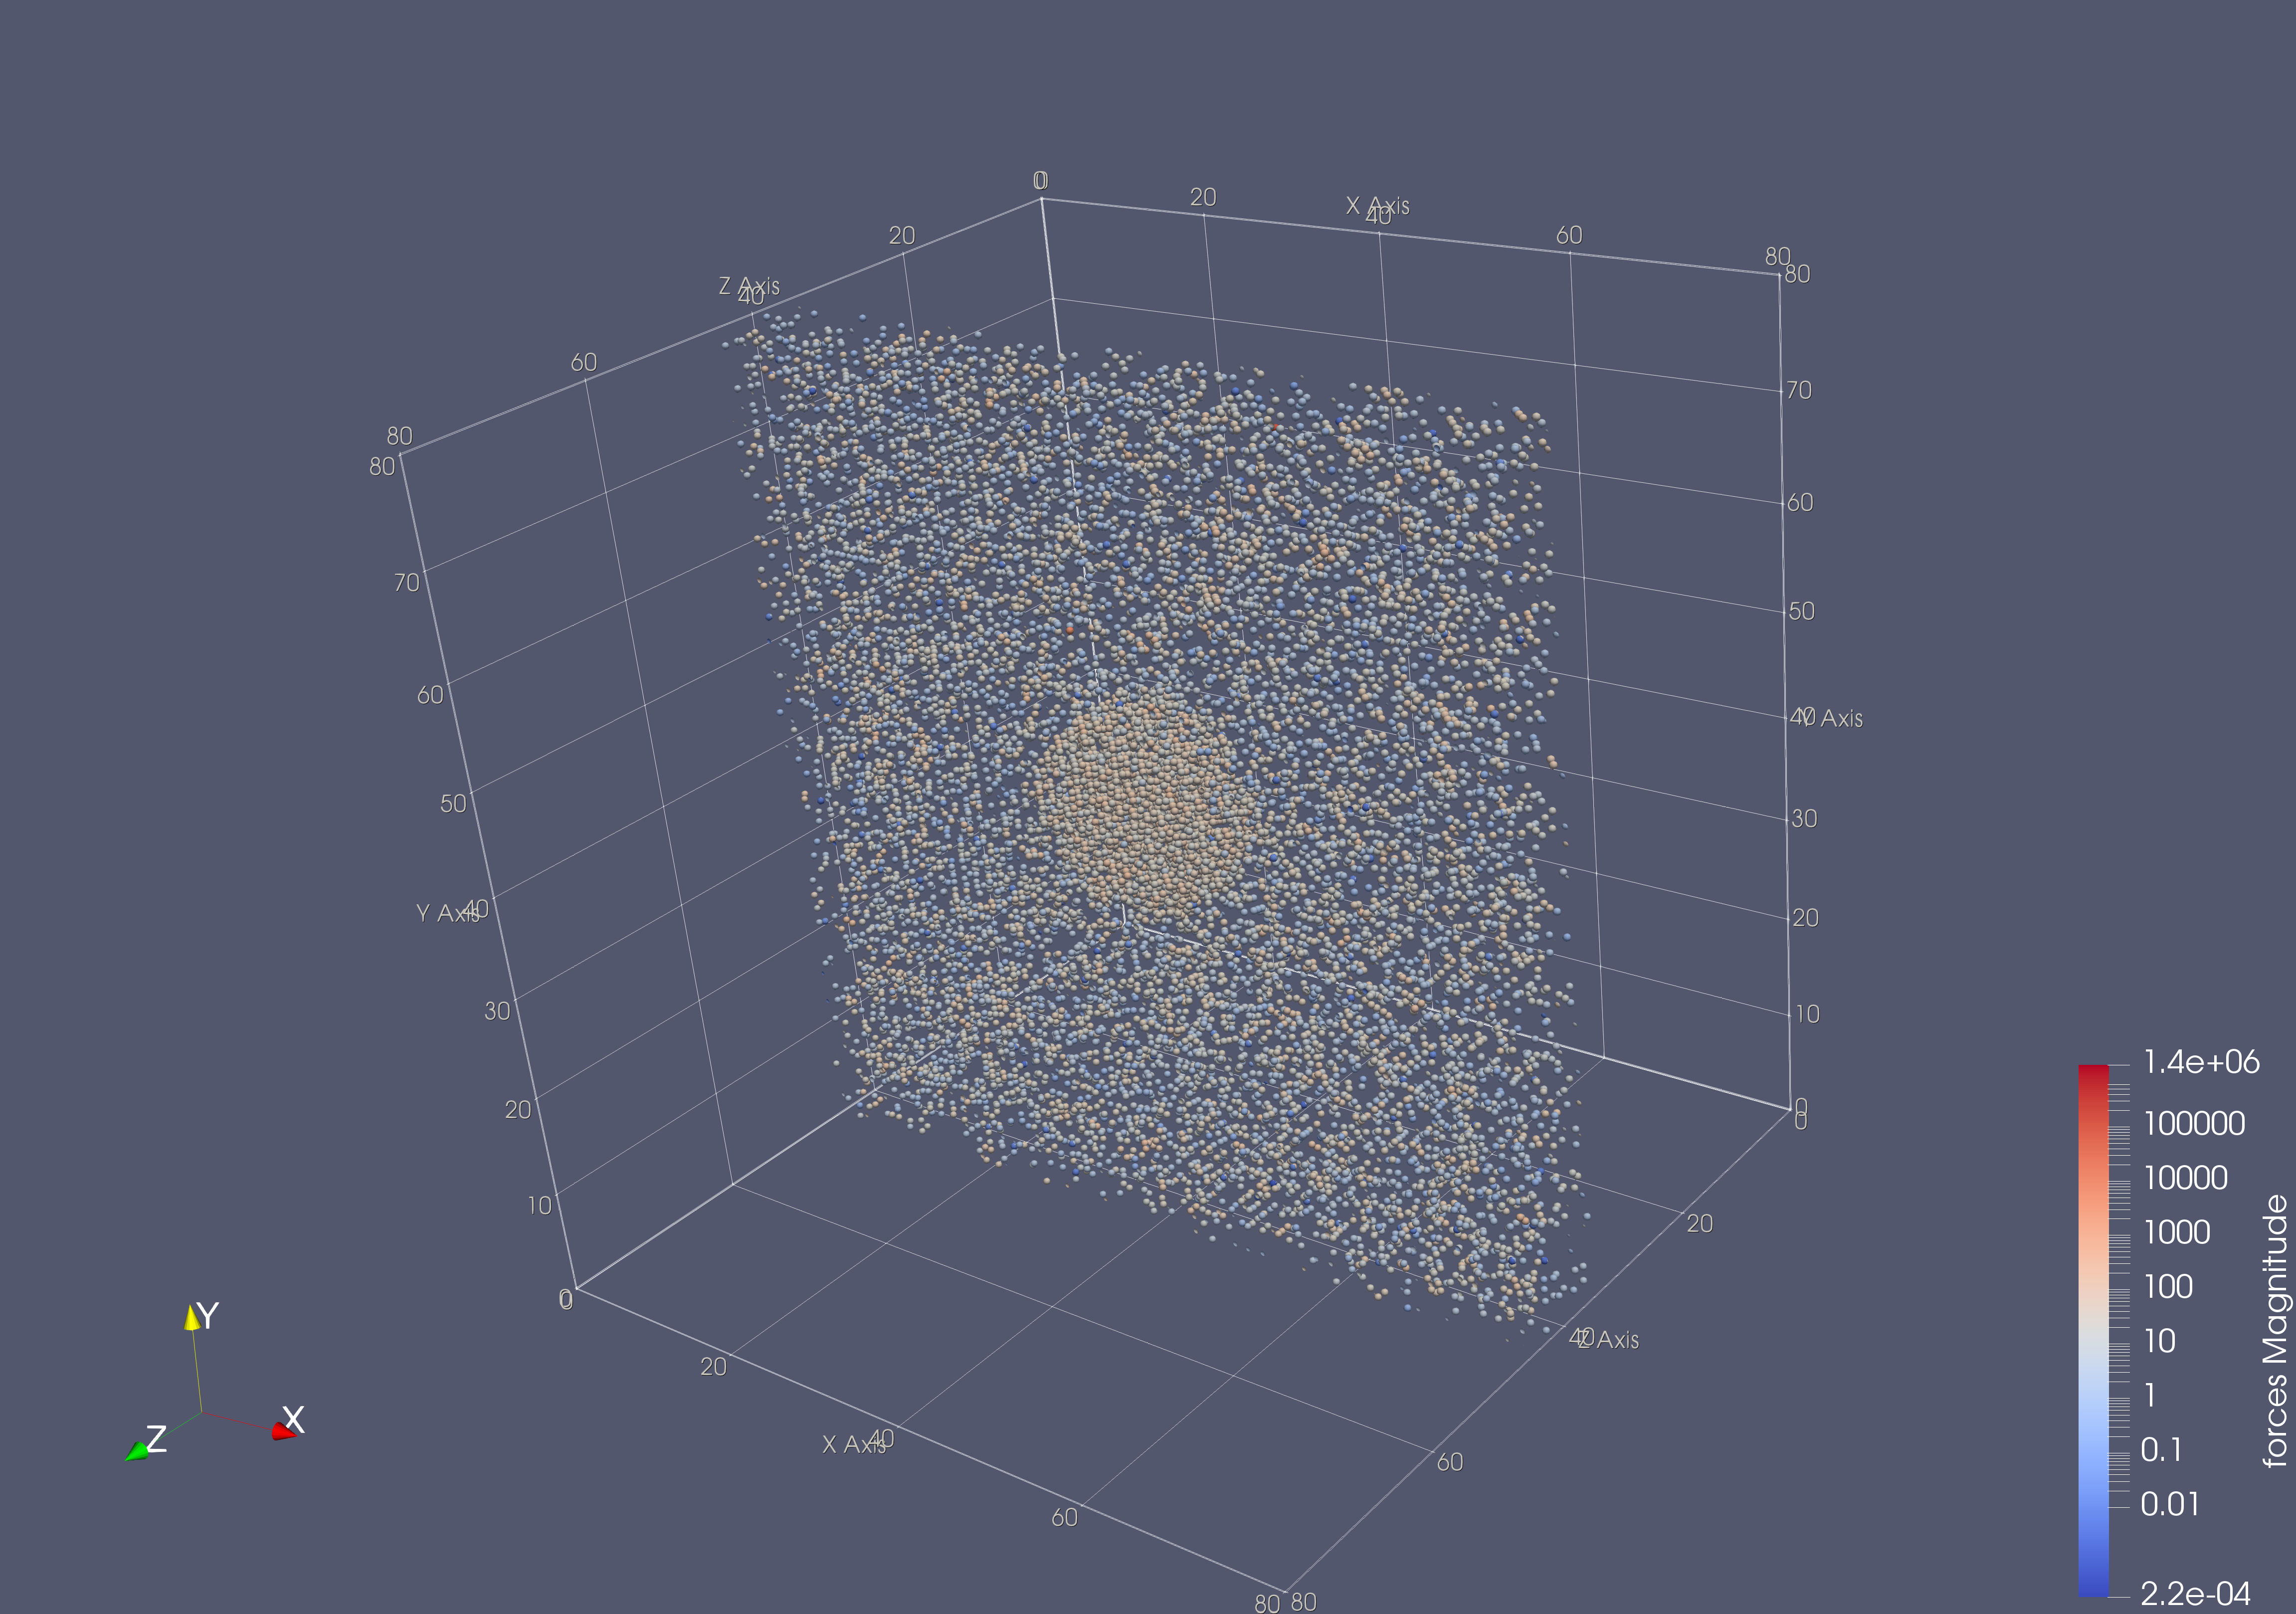
\includegraphics[width=.9\columnwidth]{figures/scenario_clip_rot.png}
        \caption[Example Figure]{Some Caption. Always also include a source if it wasn't created by you!\\
            \tiny{Source: \cite{gratl17task}}}
        \label{fig:exampleLabel1} % labels always have to be placed after the caption
    \end{figure}

    \columnbreak    % start next column

    \begin{figure}[H]
        \centering
        \begin{tikzpicture}
            \node[anchor=south west,inner sep=0] (image) at (0,0) {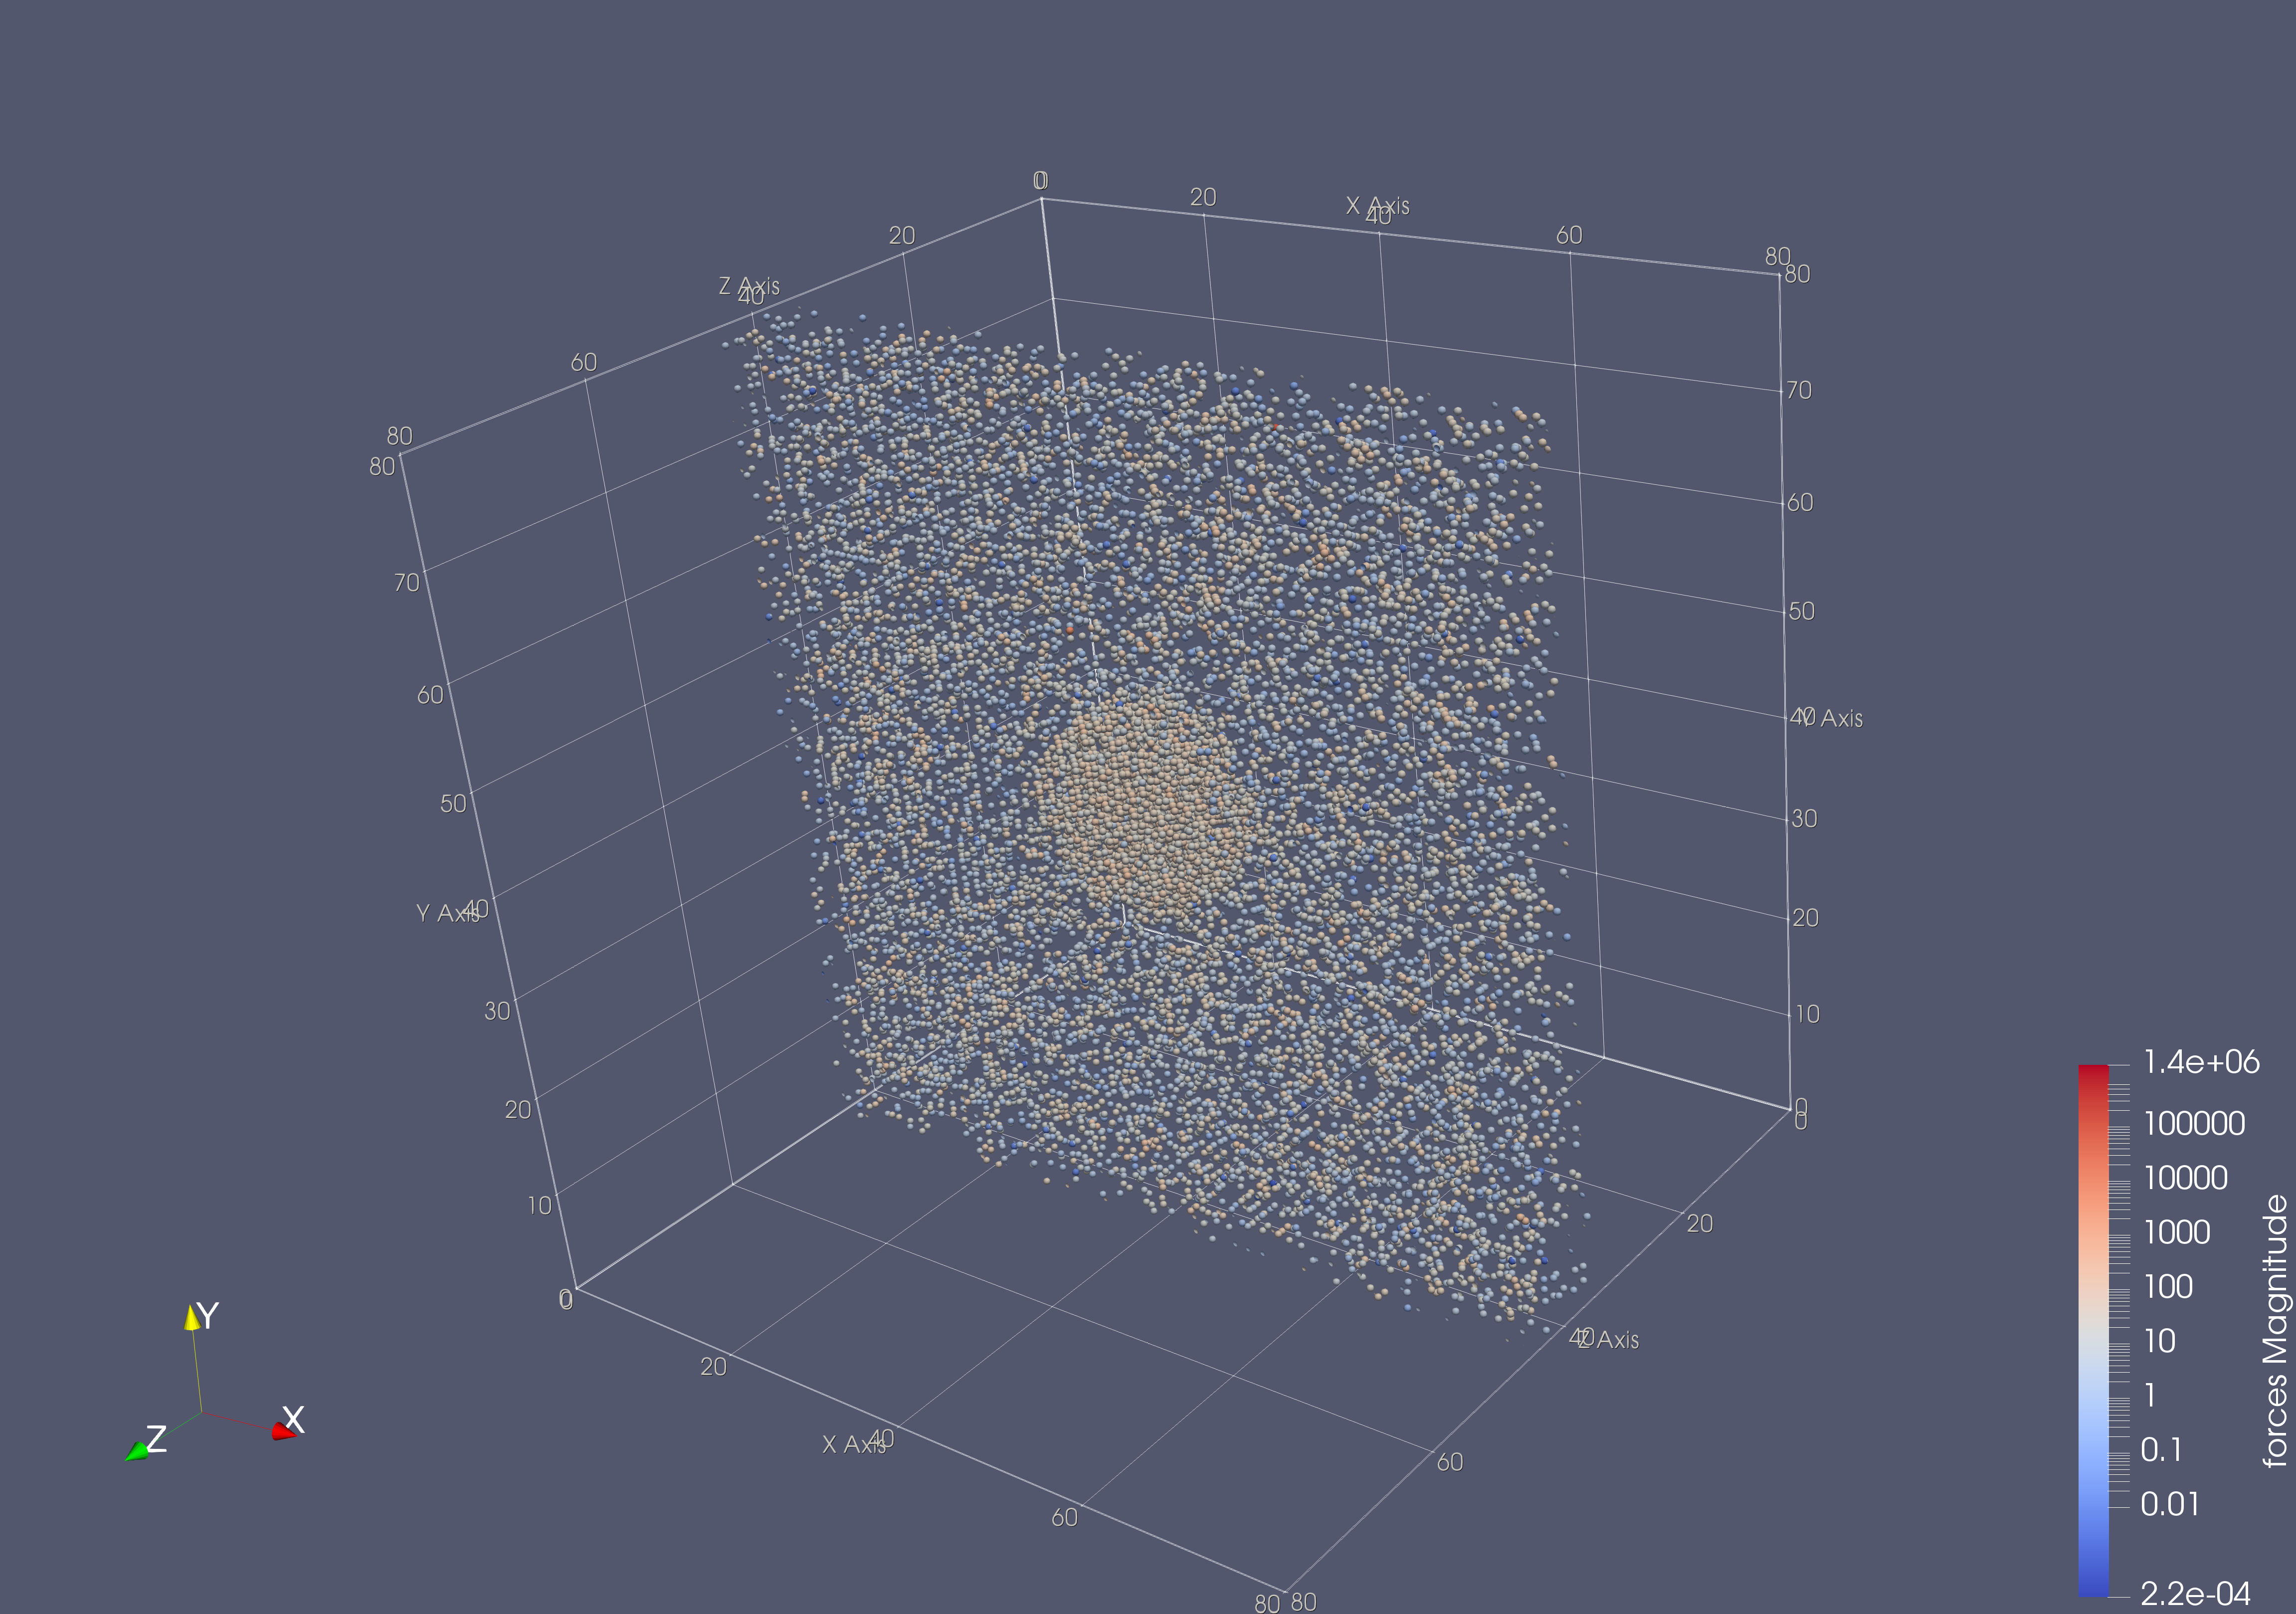
\includegraphics[width=.9\columnwidth]{figures/scenario_clip_rot.png}};
            \begin{scope}[x={(image.south east)},y={(image.north west)}]
                \draw[red, thin,rounded corners] (.42,.42) rectangle (.58,.6);
            \end{scope}
        \end{tikzpicture}
        \caption[Figure with tikz]{Figures can be drawn on or completely generated with tikz.}
        \label{fig:exampleLabel2}
    \end{figure}
\end{multicols}

\paragraph{Subfigures}
If grouping of several pictures seems reasonable, think about using subfigures. This often comes in handy with plots.

\begin{figure}[H]
    \centering
    \begin{subfigure}[b]{0.33\textwidth}
        \includegraphics[width=\textwidth]{example-image-a}
        \caption{example-image-a}
        \label{fig:example-image-a}
    \end{subfigure}
    \begin{subfigure}[b]{0.33\textwidth}
        \includegraphics[width=\textwidth]{example-image-b}
        \caption{example-image-b}
        \label{fig:example-image-b}
    \end{subfigure}
    \begin{subfigure}[b]{0.33\textwidth}
        \includegraphics[width=\textwidth]{example-image-c}
        \caption{example-image-c}
        \label{fig:example-image-c}
    \end{subfigure}
    \caption{One caption to describe them all.}
\end{figure}

\subsection{How to Algorithm}

\begin{figure}
    \begin{algorithm}[H]

        % Define custom keywords
        \SetKwFunction{KwNot}{not}
        % Define custom Functions
        \SetKwFunction{Fissorted}{is\_sorted}
        \SetKwFunction{Fbogosort}{bogosort}
        \SetKwFunction{Fshuffle}{shuffle}
        \SetKwProg{Fn}{Function}{:}{}
        \KwIn{\tabto{2cm}data array}
        \KwOut{\tabto{2cm} data sorted}
        \BlankLine

        \tcp{Checks if array is sorted}
        \Fn{\Fissorted{data}}{
            \For{i $\leftarrow$ 0 \KwTo data.size() - 1}{
                \label{algo:for}            % labels can also be put in the algorithm
                \If{data[i] $>$ data[i+1]}{
                    \Return false
                }
            }
            \Return true
        }

        \tcp{actual algorithm}
        \Fn{\Fbogosort{data}}{
            \While{\KwNot \Fissorted{data}}{
                random.\Fshuffle{data}
            }
        }

        \caption[Bogosort]{Bogosort}
        \label{algo:example}
    \end{algorithm}
    \caption{some description what is happening}
\end{figure}

\clearpage

\subsection{How to Code}
\begin{lstlisting}[style=eclipse-cpp, caption=General form of a typical runner() function., label=code:runner]
void runner(int type, void *data){
    switch(type)
        case taskType1:
            // do stuff using data
        case taskType2:
            // do other stuff using data
}
\end{lstlisting}

\subsection{How to Table}
\begin{table}[H]
    \begin{tabularx}{\columnwidth}{L | C | R}
        \hline
        \hline
        bla left                                       & bla centered\newline over two lines & bla right                                       \\
        \hline
        bla left                                       & bla centered                        & \multirow[c]{2}{\hsize}{cell spanning two rows} \\
        \cline{1-2}
        \multicolumn{2}{c|}{cell spanning two columns} &                                                                                       \\
    \end{tabularx}
    \caption[Some Table]{Fancy table that can contain line breaks and extended cells.}
    \label{tab:example}
\end{table}